
\documentclass{article}
\usepackage{graphicx}
\graphicspath{{images/}}
\usepackage{hyperref}
\usepackage{listings}

\title{TP 4A - Génie Logiciel
Programme Java intégrant modélisation UML, versionning (git)
et tests unitaires (Junit)
}
\author{Mathis Vaugeois - Tanguy Moriceau -  Faustine Guillou}
\date{January 2023}

\begin{document}

\maketitle
\tableofcontents

\newpage
\section{Introduction}

\subsection{Context}
résumé pdf
\subsection{Git}
explication installation github(mathis)
\newpage
\section{Cahier des charges}



1.Pour réaliser le diagramme de Classe, nous avons d'abord travaillé sur feuille et nous l'avons mis au prope en utilisant InkScape. 
Nous avons décider de créer un seul type Compte, avec compte courant et compte épargne deux entités différentes de Compte, car ils ont tous les deux les mêmes attributs.
Compte dépend entièrement de Dosier Bancaire, donc si le dossier bancaire est supprimé, les comptes le seront aussi.
\begin{figure}[h]
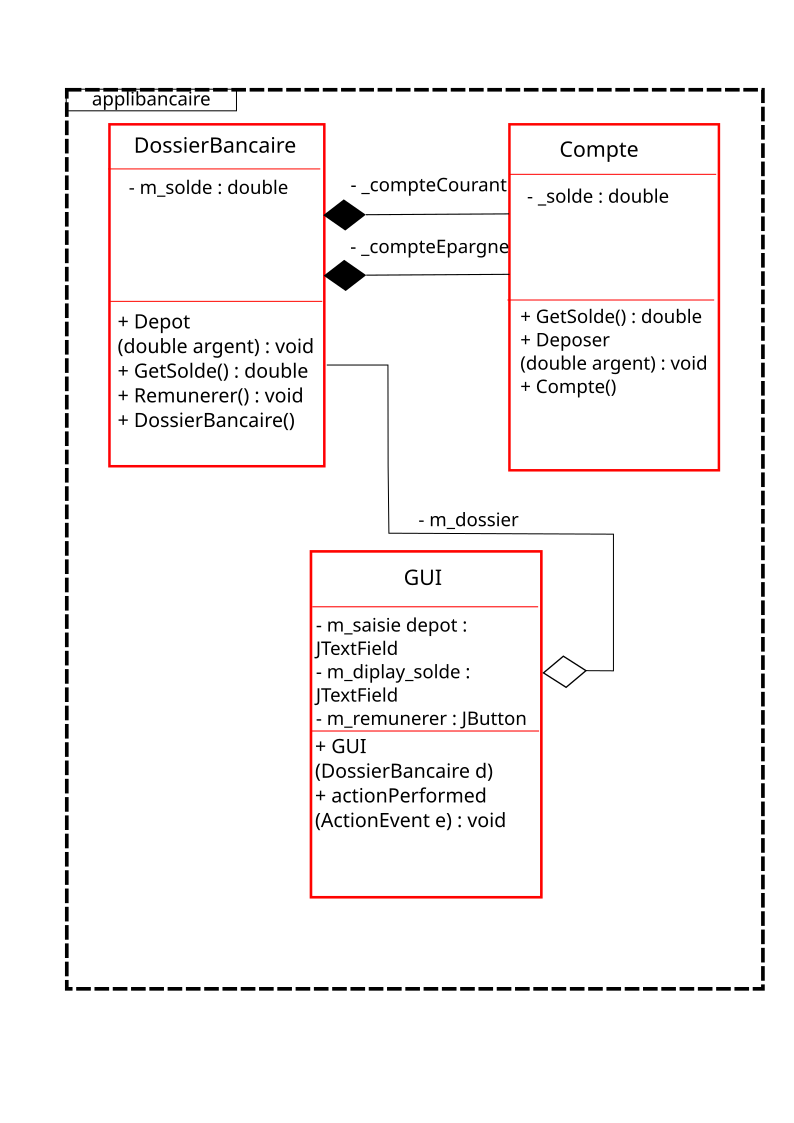
\includegraphics[width=0.8\textwidth]{diagrammeClasse.png}
\end{figure}
\newline
\newpage

2.Nous avons ensuite réalisé un diagramme de Séquence. Il débute par le main,qui initialise DossierBancaire. Pour décider des actions, DossierBancaire dépend du GUI, c'est donc par ce dernier que se lance tous les ordres.
Le premier ordre est déposer(). Via le GUI, le dépot se lance, DossierBancaire dépose sur Compte Courant et Compte Epargne.
Pour rémunérer, on récupère d'abord le solde du compte avant de prélever.
Pour le retrait, il y a double situations. Si l'argent est suffisant, on retire, si il ne l'est pas, rien ne se passe.
Pour effectuer des retraits sur le compte, nous n'avons pas créé une fonction. Nous réutilisns déposer mais en utilisant un chiffre négatif dont la valeur absolue est égale à la valeur du retrait.
%\begin{figure}[h]
%\includegraphics[width=0.8\textwidth]{diagrammeSequence.png}
%\end{figure}

3. En plus des deux diagrammes précédents, nous pourrions aussi proposer un diagramme d'objets. Le voici donc:



\begin{figure}[h]
\includegraphics[width=0.8\textwidth]{diagrammeObj.png}
\end{figure}

Il permet de rapidement voir tous les objets intervenant dans cette situation: le main, le GUI, le dossier banaire et les deux types de compte.


\newpage
\section{Code de départ}


Question 3
\newline


Après avoir ouvert le projet, nous avons récupéré les commandes données dans le README, cependant cela ne fonctionnait pas.
\newline

\begin{figure}[h]

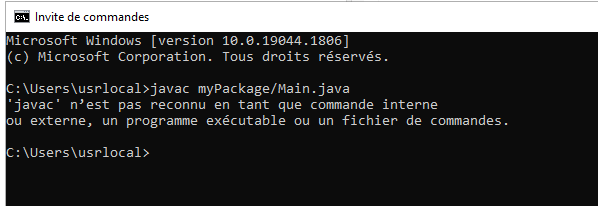
\includegraphics[width=1\textwidth]{erreurjavac.png}
\caption{Erreur de commande}
\end{figure}

 Le problème est que javac n'était pas reconnu en commande interne. Pour résoudre ce problème, nous avons ajouté javac au PATH.
 Nous avons ouvert la page Modifier les variables d'environnement dans le panneau de configuration.

\begin{figure}[h]

\includegraphics[width=0.8\textwidth]{Annotation 2023-01-10 143053.png}
\end{figure}

Ensuite nous avons ouvert l'onglet variables d'environnement et avons modié le PATH de l'utilisateur usrlocal.

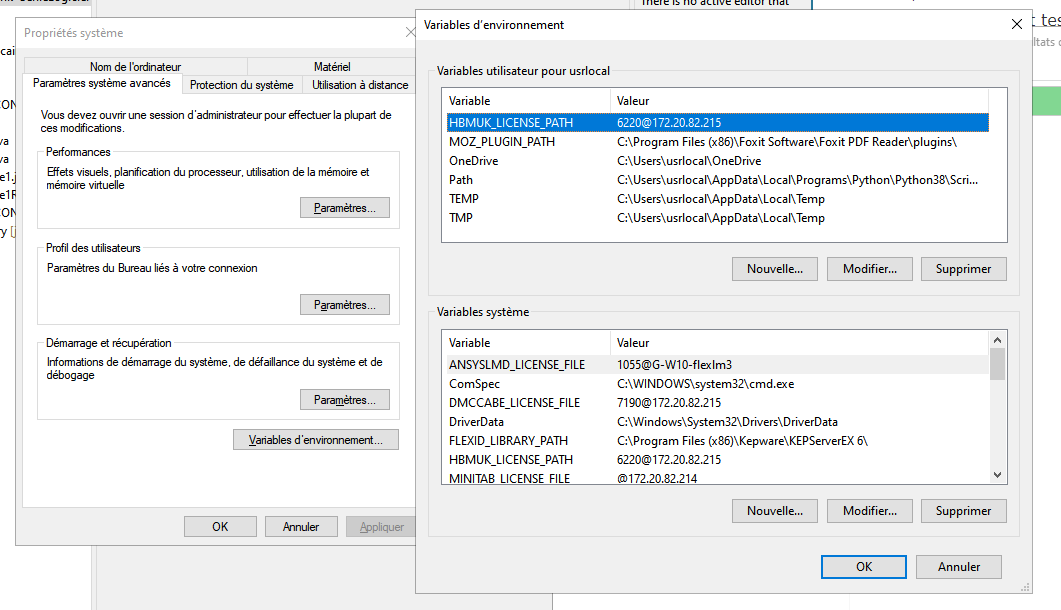
\includegraphics[width=0.8\textwidth]{Annotation 2023-01-10 143100.png}


Pour cela, nous avons du trouver le chemin de javac. Pour le trouver, nous avons tapé javac.exe dans l'explorateur de commande et avons trouvé que son chemin est C:/Program Files/Java/jdk-10.0.2/bin/javac.exe.
Nous avons ajouté le chemin du dossier dans lequel se trouve javac au PATH.


\begin{figure}[h]
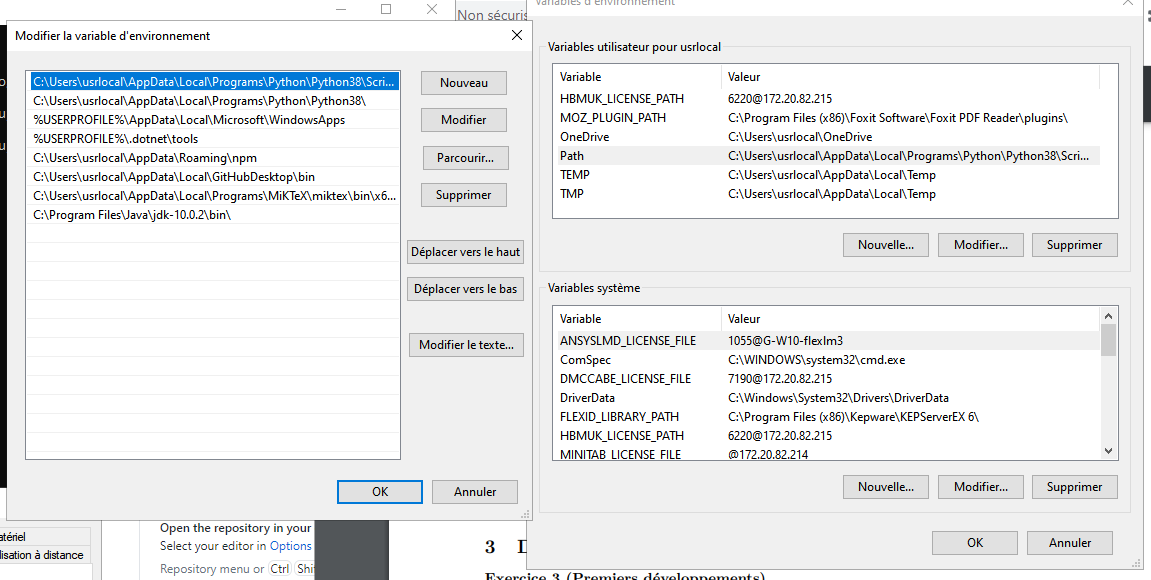
\includegraphics[width=0.8\textwidth]{Annotation 2023-01-10 145746.png}
\end{figure}
Ensuite nous avons pu relancer avec succès la commande compilation.
\begin{figure}[h]
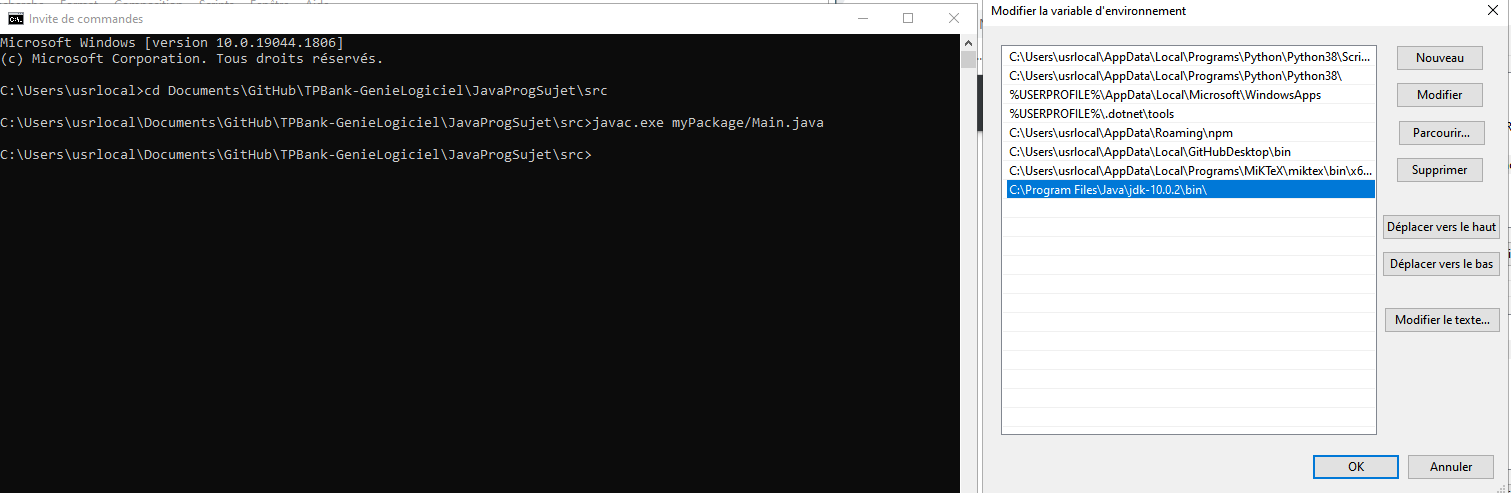
\includegraphics[width=0.8\textwidth]{Annotation 2023-01-10 145813.png}
\end{figure}

Si nous n'avions pas ajouté le chemin de javac aux path des variables d'utilisateurs, nous n'aurions pas pu utiliser la commande telle quelle. Il aurait fallu indiquer tout le chemin de javac.exe, ce qui est beaucoup plus long.
Après la compilation, le programme a pu s'éxécuter sans problème.

\newline
Question 4
\newline

La compilation et l'exécution des tests fonctionnent de manière similaire à celle du Main.
Nous avons tout d'abord récupéré la commande de compilation.

	
\begin{lstlisting}
javac -cp "C:\Program Files (x86)\eclipse\plugins
\org.junit_4.11.0.v201303080030\junit.jar";"C:\Program Files 
(x86)\eclipse\plugins\org.hamcrest.core_1.3.0.v201303031735.jar" 
tests\MyTest1.java tests\MyTest2.java ... etc...
\end{lstlisting}
Cette commande n'a pas fonctionnée.
Premièrement les chemins donnés étaient incorrects. De plus il fallait ajouter tous les fichiers tests.
La commande est donc devenue :
\begin{lstlisting}
javac -cp "C:\eclipse\plugins\org.junit_4.13.2.v20211018-1956.jar";
"C:\eclipse\plugins\org.hamcrest.core_1.3.0.v20180420-1519.jar" 
tests\MyTest1.java tests\MyTest2.java tests\MyTestSuite1.java 
tests\MyTestSuite1Runner.java myPackage\DossierBancaire.java
\end{lstlisting}

Ensuite, nous avons exécuté les testes avec la commade :
\begin{lstlisting}
    C:\Users\usrlocal\Desktop\JavaProgSujet\src>java -cp 
    "C:\Program Files (x86)\eclipse\plugins\
    org.junit_4.11.0.v201303080030\junit.jar";
    "C:\Program Files (x86)\eclipse\plugins\
    org.hamcrest.core_1.3.0.v201303031735.jar"; tests/MyTestSuite1Runner
\end{lstlisting}

Comme la commande précéente, celle-ci n'a pas fonctionné. Les chemins étaient incorrects. La correction de la commande donne :

\begin{lstlisting}
    C:\Users\usrlocal\Desktop\JavaProgSujet\src>java -cp 
    "C:\eclipse\plugins\org.junit_4.13.2.v20211018-1956.jar"
    "C:\eclipse\plugins\org.hamcrest.core_1.3.0.v20180420-1519.jar"
    tests/MyTestSuite1Runner
\end{lstlisting}
\newpage
\section{Développement}

\subsection{Exercice 3 - Premiers développements}
1. Nous avions déjà créé le dépôt git au tout début, via GitHub.

2.

3.
En premier lieu, nous avons retirés les tests inutiles. Nous avons déplacé les autres dans un fichier JUnit Teste Case que nous avons nommé "TestDossierBancaire". De plus, nous avons écris des tests supplémentaires pour tester les fonctionnalités de la classe DossierBancaire. Nous avons rajouté les tests 2,3 et 4. Nous avons ensuite renommé le fichier TestsSuites.
Voici le code du fichier de tests.

\begin{lstlisting}
   package tests;

import static org.junit.Assert.*;

import org.junit.Test;

import myPackage.DossierBancaire;

public class TestsSuite
{
	@Test  
	public void test1() 
	{
		DossierBancaire dossier = new DossierBancaire();
		dossier.deposer(100);
		assertEquals(100, dossier.get_solde(), 0);
	}
	
	
}
\end{lstlisting}
4.

5.
Une classe Compte a été créée. Celle-ci contient un solde (privé), ainsi qu'un constructeur et deux méthodes permettant de récupérer
le montant de ce solde, ainsi que de déposer de l'argent sur le compte.
\begin{lstlisting}
    package myPackage;

public class Compte
{
	private double solde;
	
	public Compte() 
	{
		solde = 0;
	}
	
	public double getSolde() 
	{
		return solde;
	}
	
	public void deposer(double somme) 
   
	{
		solde += somme;
	}
}
\end{lstlisting}
Un attribut de type Compte a été ajouté au dossier bancaire (compteCourant), permettant d'accéder aux comptes.
\begin{lstlisting}
    private double m_solde;
	private Compte _compteCourant;
	
	
    public DossierBancaire()
    {
    	m_solde=0;
    	Compte _compteCourant = new Compte();
    	
    }
\end{lstlisting}
La fonction déposer a été développée.
\begin{lstlisting}
    public void deposer(double argent)
    {
    	m_solde += argent;
    	_compteCourant.deposer(argent);
    }
\end{lstlisting}
Nous avons de plus rajouté une méthode avec d'accéder au compte couant.

\begin{lstlisting}
public Compte getCompteCourant()
    {
    	return _compteCourant;
    }
\end{lstlisting}


Ensuite, nous avons développé des tests pour ces changements.
\begin{lstlisting}

	
	@Test  
	public void test2() 
	{
		DossierBancaire dossier = new DossierBancaire();
		dossier.deposer(42);
		assertEquals(42, dossier.getCompteCourant().getSolde(), 0);		
	}
}
\end{lstlisting}


6.
Un attribut de type Compte a été ajouté au dossier bancaire (compteEpargne), permettant d'accéder aux comptes.
\begin{lstlisting}
    private double m_solde;
	private Compte _compteCourant;
	private Compte _compteEpargne;
	
    public DossierBancaire()
    {
    	m_solde=0;
    	Compte _compteCourant = new Compte();
    	Compte _compteEpargne = new Compte();
    }
\end{lstlisting}
La fonction déposer a été modifiée, pour inclure le compte épargne.
\begin{lstlisting}
     public void deposer(double somme)
    {
    	m_solde += somme;
    	_compteCourant.deposer(0.4 * somme);
    	_compteEpargne.deposer(0.6 * somme);
    }
\end{lstlisting}
Le dossier bancaire contient aussi désormais une fonction de rémunération à taux fixe, qui dépose de l'argent sur le compteEpargne.
\begin{lstlisting}
    public void remunerer()
    {
    	double somme = _compteEpargne.getSolde();
    	somme = 0.032 * somme;
    	_compteEpargne.deposer(somme);
    }
}
\end{lstlisting}
Nous avons aussi ajouté une méthode pour accéder au compte épargne.
\begin{lstlisting}
public Compte getCompteEpargne()
    {
    	return _compteEpargne;
    }
    
\end{lstlisting}

Ensuite, nous avons développé des tests pour ces changements.
\begin{lstlisting}
@Test  
	public void test3() 
	{
	   DossierBancaire dossier = new DossierBancaire();
	   dossier.deposer(100);
      assertEquals(60, dossier.getCompteEpargne().getSolde(), 0);	
	   dossier.remunerer();
	   assertEquals(61.92, dossier.getCompteEpargne().getSolde(), 0);	
	}
\end{lstlisting}


7.

Pour tagger cette version, nous avons fait un clic-droit sur la ersion en question dans l'history, et nous avons cliqué sur create tag.

8.

et 9.
Faisables avec GitDesktop.


\subsection{Exercice 4 - Fusion}

1.
Afin de répondre à cette question, nous avons légèrement modié la classe DossierBancaire en ajoutant des commentaires.
\begin{lstlisting}
        package myPackage;

public class Compte
{
	private double solde;
	
	public Compte() //constructeur du compte bancaire
	{
		solde = 0;
	}
	
	public double getSolde() //renvoie le solde du compte
	{
		return solde;
	}
	
	public void deposer(double somme) //dépose de l'argent
   
	{
		solde += somme;
	}
}
\end{lstlisting}
\begin{figure}[h]
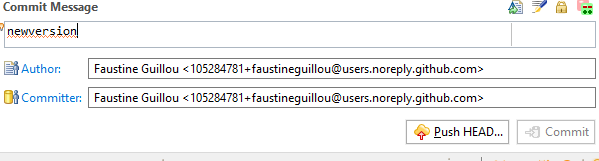
\includegraphics[width=0.8\textwidth]{commit.png}
\end{figure}
2.
Faisable avec GitDekstop. Amélioration de la structure du code précédemment réalisée (lors de l'initialisation du projet). Documentation enrichie.

3.
Documentation enrichie (commentaires).

4.
Faisable avec GitDesktop. 

5.
Tests unitaires OK et GUI OK.

\newpage
\subsection{Exercice 5 - Tests}
1.
Une fonction de retrait a été ajoutée à la classe DossierBancaire et permet de retirer de l'argent du compteCourant, avec vérification du 
solde préalablement à l'opération.

2.
Tests Junit mis en place pour tester le bon fonctionnement de l'implémentation.
\begin{lstlisting}
    @Test  
	public void test4()
	{
		DossierBancaire dossier = new DossierBancaire();
		dossier.deposer(100);
		dossier.retrait(30);
		assertEquals(10, dossier.getCompteCourant().getSolde(), 0);
	}
\end{lstlisting}

3.
Nous avons modifié l'interface GUI.

\begin{lstlisting}
    public class GUI implements ActionListener 
{
	private DossierBancaire m_dossier;
	private JTextField m_saisie_depot;
	private JTextField m_display_solde;
	private JButton m_remunerer;
	private JTextField m_saisie_retrait;

 //ajout du JTextField m_saisie_retrait
	
\end{lstlisting}
\begin{lstlisting}
     //Element saisie retrait
        m_saisie_retrait = new JTextField (20);
        m_saisie_retrait.addActionListener(this);


       frame.getContentPane().add(m_remunerer); 
        frame.getContentPane().add(new JLabel("Retrait"));
        frame.getContentPane().add(m_saisie_retrait);

        if( e.getSource() == m_saisie_retrait )
    	{
    		double retrait_value=Double.parseDouble
            (m_saisie_retrait.getText());
    		m_dossier.retrait(retrait_value);
    		m_saisie_retrait.setText("");
    	}
    	m_display_solde.setText(Double.toString(m_dossier.get_solde())); 
\end{lstlisting}

4. Après avoir fait ces nouvelles modifications, nous avons commit sur GitHub Desktop. Ensuite, nous avons push. Dans l'interface history énumérant tous les commit, nous avons fait un clic droit sur le dernier et avons sélectionné create tag.

Tout au long de la partie concernant Eclipse, nous avons alterné entre Eclipse et GitHub Desktop pour commit nos changements. Les deux fonctionnent tout aussi bien l'un que l'autre. La seule différence entre les deux interfaces sont les fichiers commit. Eclipse ne commit que le projet lui-même. Avec Github, nous pouvons commit en même temps d'autres fichiers faisant parti du dépôt mais étant en dehors du projet Eclipse. C'est cette difféence qui a déterminé l'alternance entre ces deux interfaces.
\section*{Référence}
\url{https://github.com/mathisvaugeois/TPBank-GenieLogiciel}

\end{document}